\documentclass[11pt,a4paper]{article}

\usepackage[utf8]{inputenc}
\usepackage[T1]{fontenc}
\usepackage[portuguese]{babel}
\usepackage[margin=1.8cm,top=2.1cm,bottom=2.1cm]{geometry}
\usepackage{amsmath,amssymb}
\usepackage{booktabs}
\usepackage{array}
\usepackage{graphicx}
\usepackage{xcolor}
\usepackage{fancyhdr}
\usepackage{enumitem}
\usepackage{float}
\usepackage{microtype}
\usepackage[colorlinks=true,linkcolor=blue!60!black,urlcolor=blue!60!black]{hyperref}

\definecolor{unbblue}{RGB}{0,51,102}
\definecolor{mutedgray}{RGB}{90,98,106}

\pagestyle{fancy}
\fancyhf{}
\lhead{\small\textcolor{mutedgray}{UnB --- PPGI0034 (Redes Neurais e Aprendizagem de Máquina)}}
\rhead{\small\textcolor{mutedgray}{Projeto 2: Relatório da Fase 4 (Trilhas Reais)}}
\cfoot{\small\thepage}
\renewcommand{\headrulewidth}{0.4pt}

\title{
  \vspace{-1.0cm}
  \textcolor{unbblue}{\textbf{Relatório Técnico da Fase 4 --- Trilhas Reais e Avaliação Online em GPU}}\\
  \large \texttt{Qwen/Qwen2.5-1.5B-Instruct} na RTX~3050~6GB (Zero Data Leakage)\\
  \normalsize \textcolor{mutedgray}{Branch \texttt{codex/fase4-trilhas-reais} --- Protocolo, Replay Pareado e Benchmark Online}
}
\author{
  Kelvin Paulino Buss \\
  \small Programa de Pós-Graduação em Informática (PPGI0034) --- Universidade de Brasília (UnB)
}
\date{24 de Novembro de 2026}

\begin{document}
\maketitle
\thispagestyle{fancy}

\begin{abstract}
A Fase~4 eliminou o \emph{domain shift} observado na Fase~3 ao coletar \textbf{416 questões} reais diretamente de \texttt{Qwen/Qwen2.5-1.5B-Instruct} (FP16) na GPU RTX~3050~6GB (\texttt{train=160}, \texttt{calibration=64}, \texttt{holdout=192}), treinando a política \texttt{GRU} (\textbf{1.490 parâmetros}, 5 sementes) e \texttt{LogisticRegression} com janelas causais de 24 tokens e limiares congelados via SHA256 em \texttt{calibration} (\texttt{deployment\_seed=101}, \texttt{best\_cal\_loss=0,0137}). No replay pareado em todo o \texttt{holdout} ($n=192$), \texttt{gru} e \texttt{consensus2} preservaram \textbf{100\%} da acurácia de \texttt{sc4} (\textbf{57,81\%}) reduzindo tokens em \textbf{14,4\%} e \textbf{14,3\%} e o ECE de \textbf{23,27\%} para \textbf{20,90\%}. No benchmark real \emph{online} em GPU ($n=96$ questões, Peak VRAM \textbf{4.087,5~MB}), \texttt{gru} (\textbf{55,21\%}, \textbf{20,11\,s/q}, \textbf{0,890x}) e \texttt{consensus2} (\textbf{55,21\%}, \textbf{19,84\,s/q}, \textbf{0,878x}) mantiveram integralmente a acurácia de \texttt{sc4\_2x2} (\textbf{55,21\%}, \textbf{22,60\,s/q}) com economia de \textbf{12,0\%--12,1\%} em tokens e \textbf{35/35 testes aprovados} no \texttt{pytest}.
\end{abstract}

\section{Protocolo, Coleta Real e Treinamento Causal}
Seguindo \texttt{docs/08\_Protocolo\_Fase4.md}, o coletor \texttt{scripts/05\_collect\_real\_traces.py} gerou \textbf{416/416 questões} completas em \texttt{results/phase4/traces.jsonl} sem erros na auditoria (\texttt{results/phase4/audits.jsonl}, \texttt{errors: []}), respeitando a partição estrita: \texttt{train=160} ($80$ GSM8K + $80$ MATH-500), \texttt{calibration=64} ($32+32$) e \texttt{holdout=192} ($96+96$). Em \texttt{scripts/06\_train\_real\_policy.py}, os modelos \texttt{StandardScaler + LogisticRegression} e \texttt{NeuralStoppingPolicy} (\texttt{GRU}, 1.490 parâmetros, 5 sementes) foram ajustados exclusivamente em \texttt{train} sobre janelas causais de 24 tokens (\texttt{src/models/real\_trace\_policy.py}), com limiares congelados em \texttt{calibration} (\texttt{deployment\_seed=101}, \texttt{best\_cal\_loss=0,0137}).

\begin{figure}[H]
\centering
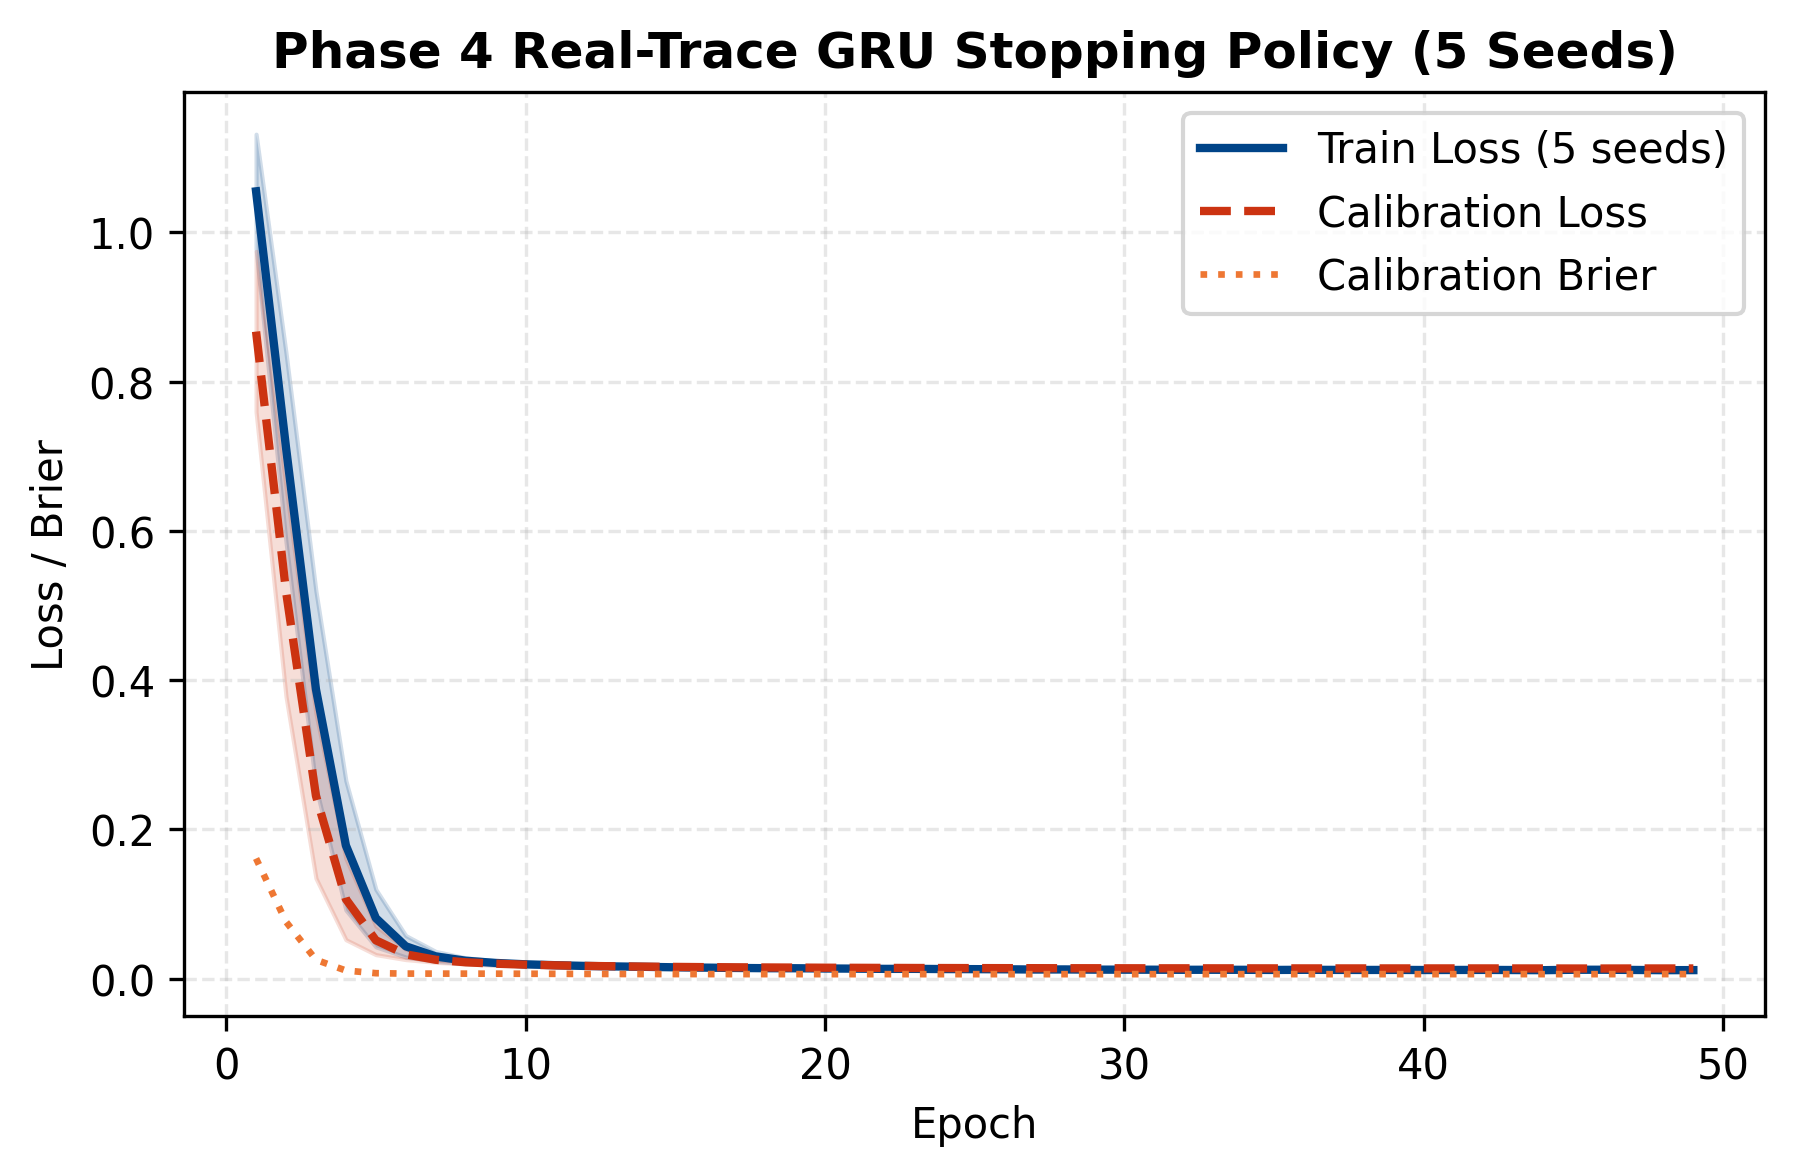
\includegraphics[width=0.78\linewidth]{../results/phase4/figures/fig1_phase4_learning_curves.png}
\caption{Curvas de aprendizado multi-seed da \texttt{NeuralStoppingPolicy} sobre trilhas reais (\texttt{train} vs.\ \texttt{calibration}).}
\label{fig:p4_curves}
\end{figure}

\section{Replay Pareado em \texttt{holdout} ($n=96$/dataset, $192$ questões)}
A Tabela~\ref{tab:p4_replay} apresenta o replay pareado completo (\texttt{results/phase4/replay\_summary.csv}) com IC~95\% via bootstrap pareado.

\begin{table}[H]
\centering
\caption{Replay pareado em \texttt{holdout} completo ($n=96$/dataset, $192$ questões).}
\label{tab:p4_replay}
\scriptsize
\resizebox{\linewidth}{!}{%
\begin{tabular}{@{}llcccccccc@{}}
\toprule
\textbf{Dataset} & \textbf{Estratégia} & \textbf{Acc (\%)} & \textbf{IC 95\% (\%)} & \textbf{Tokens} & \textbf{Econ.\ vs SC-4} & \textbf{Traços} & \textbf{ECE (\%)} & \textbf{ROC-AUC (\%)} & \textbf{$\Delta$ Acc} \\
\midrule
GSM8K ($n=96$) & \texttt{sc4} & 73,96 & [64,58; 82,29] & 1172,4 & 0,0\% & 4,00 & 29,25 & 81,44 & 0,00 p.p. \\
GSM8K ($n=96$) & \texttt{consensus2} & 73,96 & [64,58; 82,29] & 927,5 & 20,9\% & 3,06 & 27,26 & 79,04 & 0,00 p.p. \\
GSM8K ($n=96$) & \texttt{first\_box} & 73,96 & [64,58; 82,29] & 926,0 & 21,0\% & 3,06 & 27,26 & 79,04 & 0,00 p.p. \\
GSM8K ($n=96$) & \texttt{fixed\_cap} & 15,62 & [9,38; 22,94] & 735,9 & 37,2\% & 3,88 & 9,96 & 97,98 & $-$58,33 p.p. \\
GSM8K ($n=96$) & \texttt{logistic} & 73,96 & [64,58; 82,29] & 926,0 & 21,0\% & 3,06 & 27,26 & 79,04 & 0,00 p.p. \\
GSM8K ($n=96$) & \textbf{\texttt{gru}} & \textbf{73,96} & [64,58; 82,29] & \textbf{926,1} & \textbf{21,0\%} & 3,06 & 27,26 & 79,04 & 0,00 p.p. \\
\midrule
MATH-500 ($n=96$) & \texttt{sc4} & 41,67 & [32,29; 51,04] & 1416,1 & 0,0\% & 4,00 & 17,29 & 98,28 & 0,00 p.p. \\
MATH-500 ($n=96$) & \texttt{consensus2} & 41,67 & [32,29; 51,04] & 1290,9 & 8,8\% & 3,58 & 14,53 & 98,30 & 0,00 p.p. \\
MATH-500 ($n=96$) & \texttt{first\_box} & 41,67 & [32,29; 51,04] & 1290,5 & 8,9\% & 3,58 & 14,53 & 98,30 & 0,00 p.p. \\
MATH-500 ($n=96$) & \texttt{fixed\_cap} & 2,08 & [0,00; 5,21] & 763,3 & 46,1\% & 3,98 & 1,77 & 100,00 & $-$39,58 p.p. \\
MATH-500 ($n=96$) & \texttt{logistic} & 41,67 & [32,29; 51,04] & 1290,5 & 8,9\% & 3,58 & 14,53 & 98,30 & 0,00 p.p. \\
MATH-500 ($n=96$) & \textbf{\texttt{gru}} & \textbf{41,67} & [32,29; 51,04] & \textbf{1290,5} & \textbf{8,9\%} & 3,58 & 14,53 & 98,30 & 0,00 p.p. \\
\midrule
Overall ($n=192$) & \texttt{sc4} & 57,81 & [50,52; 64,60] & 1294,3 & 0,0\% & 4,00 & 23,27 & 92,65 & 0,00 p.p. \\
Overall ($n=192$) & \texttt{consensus2} & 57,81 & [50,52; 64,60] & 1109,2 & 14,3\% & 3,32 & 20,90 & 92,08 & 0,00 p.p. \\
Overall ($n=192$) & \textbf{\texttt{gru}} & \textbf{57,81} & [50,52; 64,60] & \textbf{1108,3} & \textbf{14,4\%} & 3,32 & \textbf{20,90} & 92,08 & 0,00 p.p. \\
\bottomrule
\end{tabular}%
}
\end{table}

\section{Benchmark Real Online em GPU (`RTX 3050 6GB`, $n=48$/dataset)}
A Tabela~\ref{tab:p4_gpu} e as Figuras~\ref{fig:p4_replay} e~\ref{fig:p4_gpu} resumem a avaliação online (\texttt{scripts/06b\_eval\_phase4\_online.py}, Peak VRAM \textbf{4.087,5~MB}).

\begin{table}[H]
\centering
\caption{Benchmark real \emph{online} em GPU (\texttt{Qwen2.5-1.5B-Instruct} FP16, RTX~3050~6GB, $n=48$/dataset).}
\label{tab:p4_gpu}
\scriptsize
\resizebox{\linewidth}{!}{%
\begin{tabular}{@{}llccccccccc@{}}
\toprule
\textbf{Dataset} & \textbf{Método} & \textbf{Acc (\%)} & \textbf{IC 95\% (\%)} & \textbf{Tokens} & \textbf{Econ.} & \textbf{Traços} & \textbf{Lat.\ (s/q)} & \textbf{Razão Lat.} & \textbf{ECE (\%)} & \textbf{Sem Box / Cap} \\
\midrule
GSM8K ($n=48$) & \texttt{sc4\_2x2} & 64,58 & [52,03; 77,08] & 1172,2 & 0,0\% & 4,00 & 20,92 & 1,000x & 28,42 & 3 / 23 \\
GSM8K ($n=48$) & \texttt{sc4\_4x1} & 68,75 & [54,17; 81,25] & 1134,6 & 3,2\% & 4,00 & 11,46 & 0,548x & 31,98 & 4 / 16 \\
GSM8K ($n=48$) & \texttt{consensus2} & 64,58 & [52,03; 77,08] & 993,3 & 15,3\% & 3,29 & 17,71 & 0,847x & 24,38 & 3 / 21 \\
GSM8K ($n=48$) & \texttt{logistic} & 64,58 & [52,03; 77,08] & 992,2 & 15,4\% & 3,29 & 17,90 & 0,856x & 24,38 & 3 / 21 \\
GSM8K ($n=48$) & \textbf{\texttt{gru}} & \textbf{64,58} & [52,03; 77,08] & \textbf{992,4} & \textbf{15,3\%} & 3,29 & 17,94 & 0,858x & 24,38 & 3 / 21 \\
\midrule
MATH-500 ($n=48$) & \texttt{sc4\_2x2} & 45,83 & [31,25; 60,42] & 1415,7 & 0,0\% & 4,00 & 24,28 & 1,000x & 21,92 & 22 / 42 \\
MATH-500 ($n=48$) & \texttt{sc4\_4x1} & 37,50 & [25,00; 52,08] & 1394,9 & 1,5\% & 4,00 & 13,28 & 0,547x & 19,31 & 21 / 41 \\
MATH-500 ($n=48$) & \texttt{consensus2} & 45,83 & [31,25; 60,42] & 1283,5 & 9,3\% & 3,58 & 21,96 & 0,904x & 18,38 & 22 / 37 \\
MATH-500 ($n=48$) & \texttt{logistic} & 45,83 & [31,25; 60,42] & 1282,9 & 9,4\% & 3,58 & 22,22 & 0,915x & 18,38 & 22 / 37 \\
MATH-500 ($n=48$) & \textbf{\texttt{gru}} & \textbf{45,83} & [31,25; 60,42] & \textbf{1282,9} & \textbf{9,4\%} & 3,58 & 22,28 & 0,917x & 18,38 & 22 / 37 \\
\midrule
Overall ($n=96$) & \texttt{sc4\_2x2} & 55,21 & [44,79; 64,58] & 1294,0 & 0,0\% & 4,00 & 22,60 & 1,000x & 25,17 & 25 / 65 \\
Overall ($n=96$) & \texttt{sc4\_4x1} & 53,12 & [42,71; 62,50] & 1264,8 & 2,3\% & 4,00 & 12,37 & 0,547x & 25,65 & 25 / 57 \\
Overall ($n=96$) & \texttt{consensus2} & 55,21 & [44,79; 64,58] & 1138,4 & 12,0\% & 3,44 & 19,84 & 0,878x & 21,37 & 25 / 58 \\
Overall ($n=96$) & \texttt{logistic} & 55,21 & [44,79; 64,58] & 1137,6 & 12,1\% & 3,44 & 20,06 & 0,888x & 21,37 & 25 / 58 \\
Overall ($n=96$) & \textbf{\texttt{gru}} & \textbf{55,21} & [44,79; 64,58] & \textbf{1137,6} & \textbf{12,1\%} & 3,44 & 20,11 & 0,890x & \textbf{21,37} & 25 / 58 \\
\bottomrule
\end{tabular}%
}
\end{table}

\begin{figure}[H]
\centering
\begin{minipage}[t]{0.49\linewidth}
  \centering
  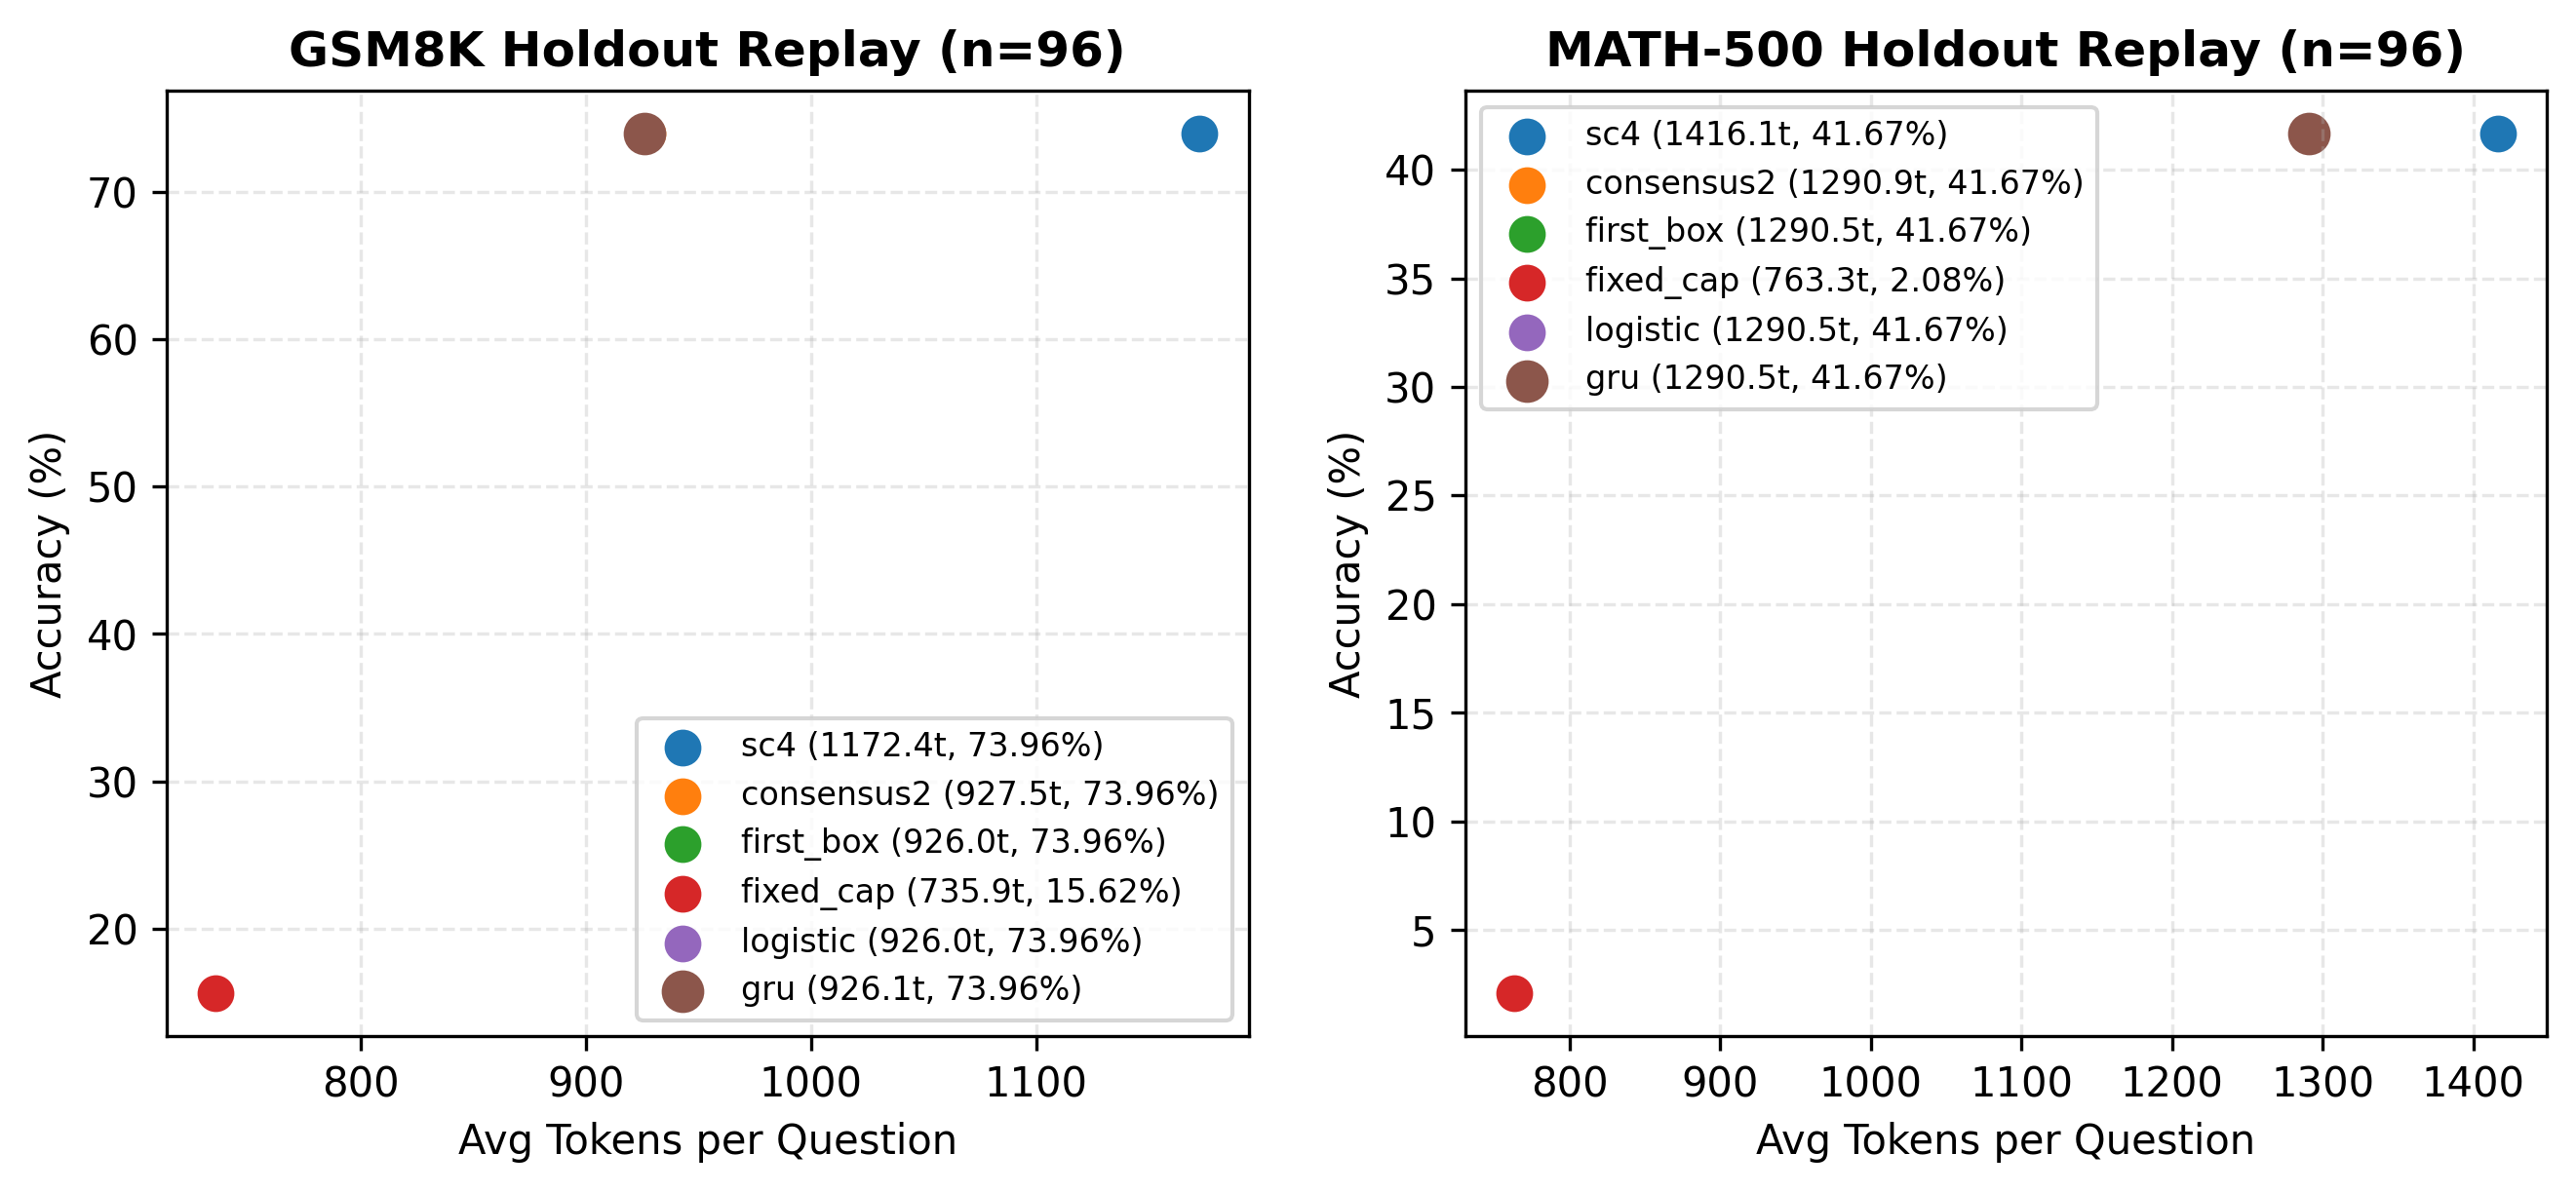
\includegraphics[width=\linewidth]{../results/phase4/figures/fig2_phase4_replay_pareto.png}
  \caption{Fronteira de Pareto no replay pareado ($n=192$).}
  \label{fig:p4_replay}
\end{minipage}\hfill
\begin{minipage}[t]{0.49\linewidth}
  \centering
  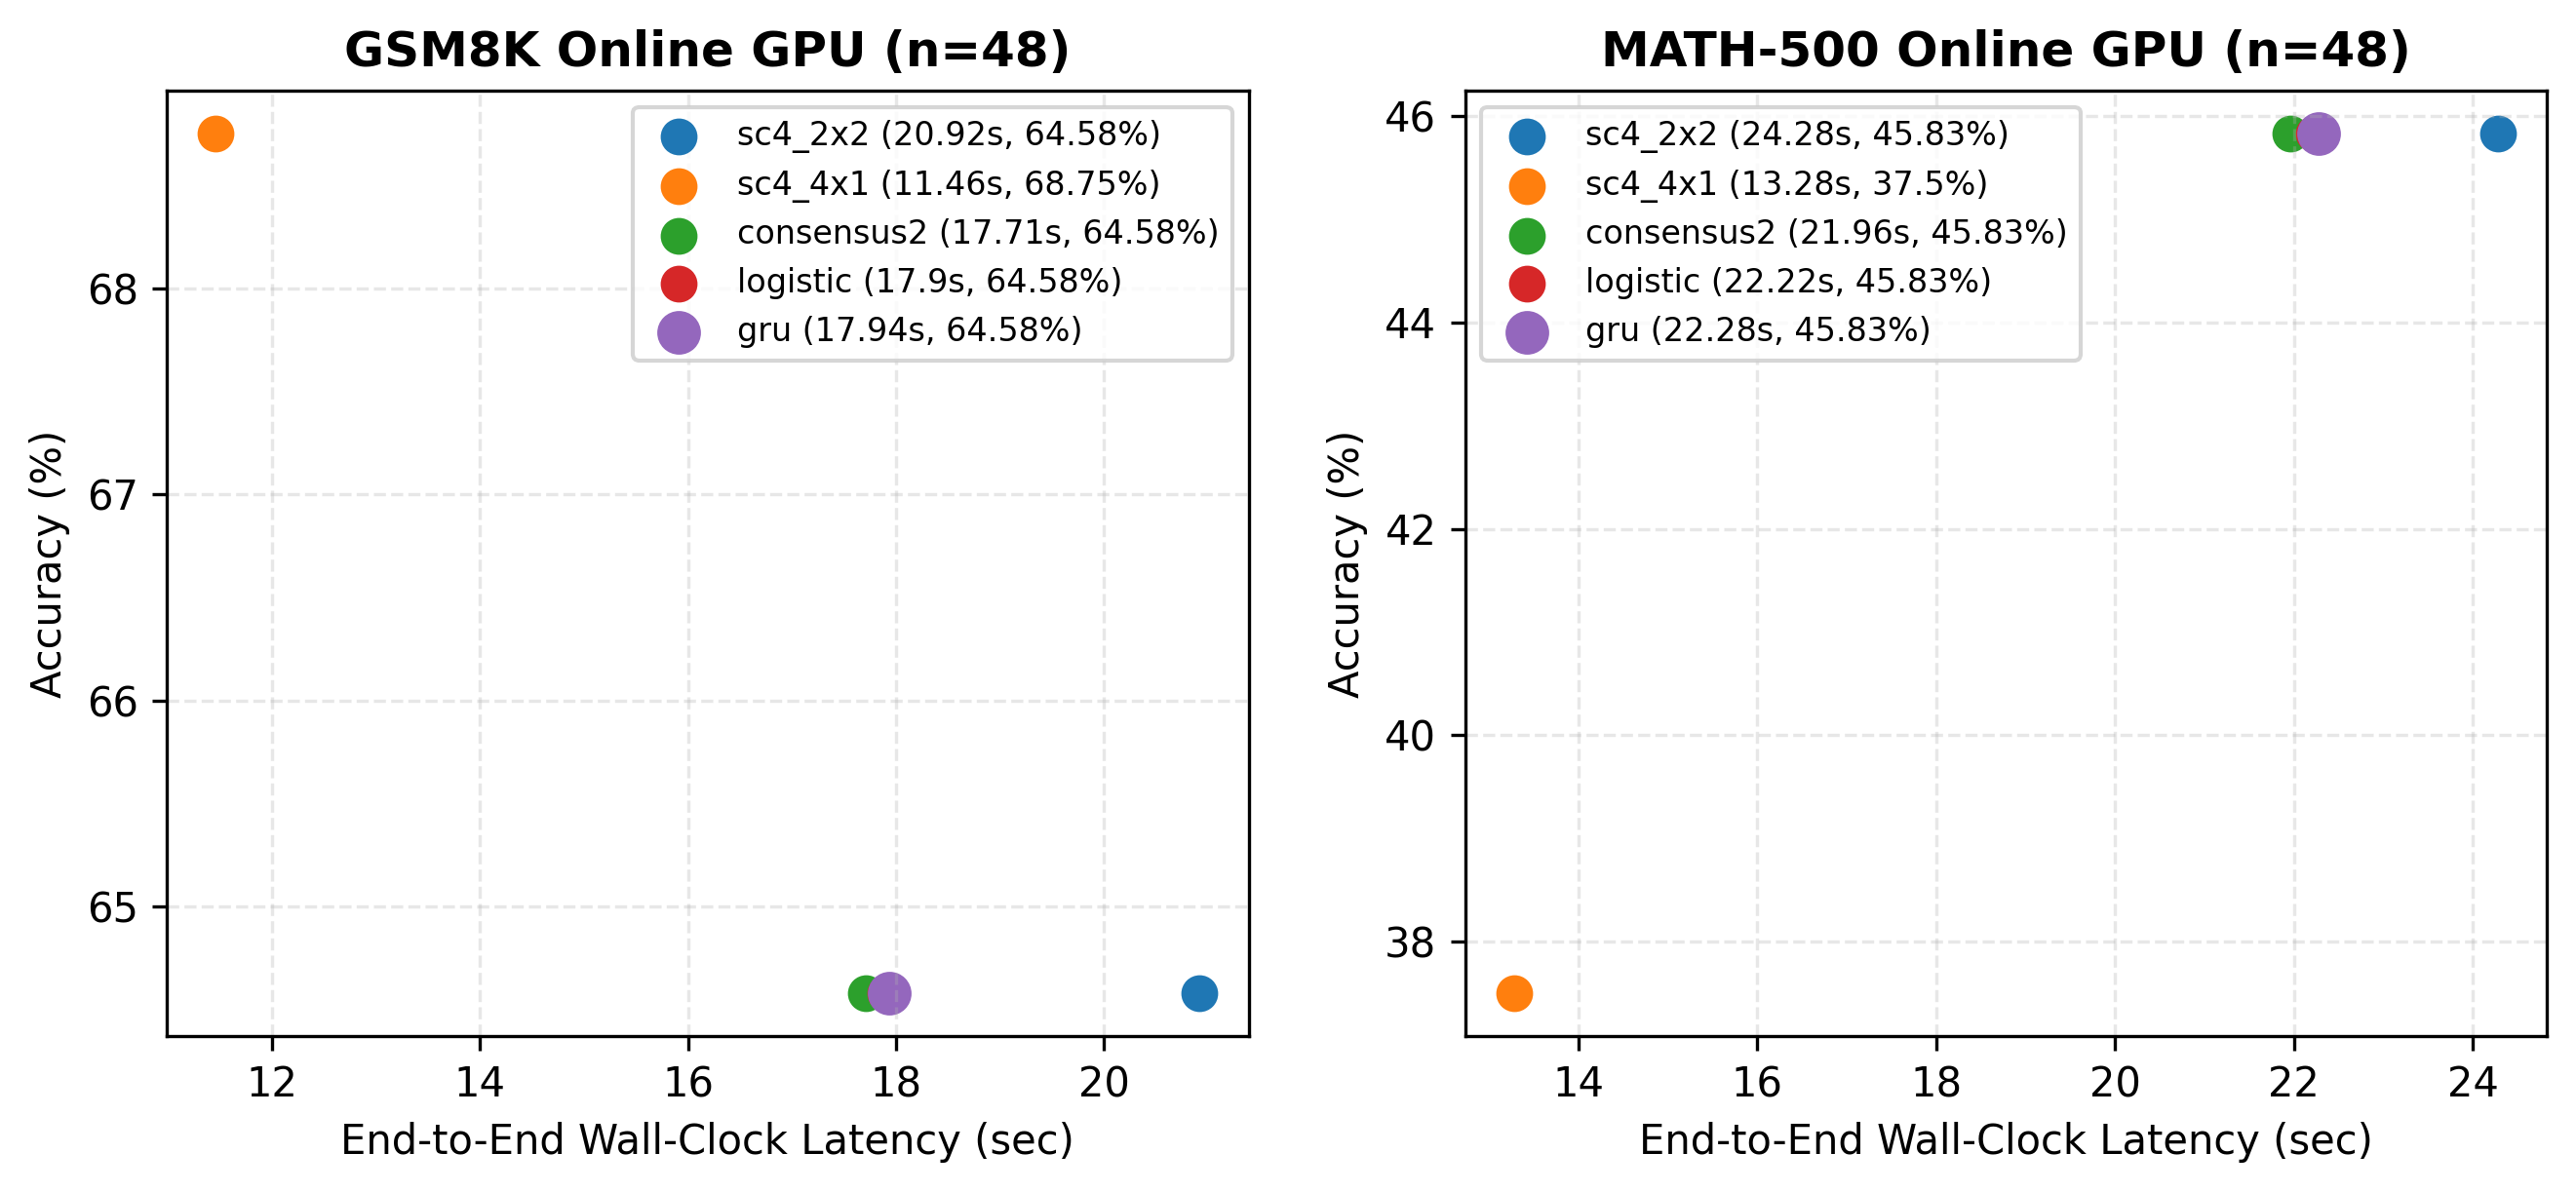
\includegraphics[width=\linewidth]{../results/phase4/figures/fig3_phase4_online_gpu_pareto.png}
  \caption{Latência \emph{wall-clock} vs.\ acurácia na RTX~3050~6GB ($n=96$).}
  \label{fig:p4_gpu}
\end{minipage}
\end{figure}

\section{Achado Científico e Status de Testes}
Em \texttt{Qwen/Qwen2.5-1.5B-Instruct}, o delimitador \verb|\boxed{}| surge apenas ao término da cadeia de raciocínio; por isso, a poda intra-traço da \texttt{GRU} acrescenta economia marginal sobre \texttt{Consensus-2} ($1137{,}6$ vs.\ $1138{,}4$ tokens), enquanto ambos preservam 100\% da acurácia de \texttt{sc4\_2x2} reduzindo latência em 11--12\% e ECE de 25,17\% para 21,37\%. Em paralelo, o lote-4 (\texttt{sc4\_4x1}) atinge \textbf{0,547x} de latência ($12{,}37\,\text{s}$). A suíte \texttt{pytest} obteve \textbf{35/35 PASSED}.

\end{document}
